\documentclass[CS5104-Notes.tex]{subfiles}
\begin{document}

\section{Introduction}
In machine learning, we wish to \textit{learn} the mapping between input and output without having to program it explicitly.

\begin{displayquote}
Maching learning is the field of study that gives computers the ability to learn without being explicitly programmed. - Arther Samuel.
\end{displayquote}

\begin{displayquote}
A computer program is said to learn from exerience $E$ with respect to some task $T$ and some performance measure $P$, if its performance on $T$, as measured by $P$, improves with experience $E$. - Tom Mitchell.
\end{displayquote}
\noindent
In general, most machine learning boils down to a simple prediction equation.
\begin{align}
  \hat Y &= f(X, \theta) \\
  Y &= f(X, \theta) + \varepsilon
\end{align}
where $f$ is a mathematical model for predicting $Y$ from $X$. $X$ is a list of input features that are used for prediction. They could be independent variables or some kind of predictor. $\hat Y$ is the output of the predicting model which are the predicted values. $\theta$ are the model parameters that the model tries to learn and optimise for. Finally, $\varepsilon$ is the error, which represents the difference between predicted values and desired values.

\subsection{Prediction error}
In order to measure the difference between the predicted values and actual values, the error for each data point must be measured or calculated in some way. To do this a \textbf{loss function} (cost function) is used to evaluate the quality of the model. The goal is to then try to minimise the loss function by altering the $\theta$ parameters to allow the model to make better predictions.
\n
An example of a common loss function is the squared error loss.
\begin{equation}
L(\theta) = (Y - f(X, \theta))^2
\end{equation}
The loss function serves as a way to measure the quality of prediction for the set of parameters.

\subsection{Machine learning process}
\begin{enumerate}
  \item Gather data
  \item Prepare data (data cleaning and preprocessing)
  \item Pick an algorithm (or a few different ones)
  \item Pick a set of parameters
  \item Evaluate performance of model
  \item If the performance is not good, re-evaluate by altering parameters
  \item Apply model to new/unseen data
\end{enumerate}
This is generally implemented as an optimisation process, where the loss function is minimised on each iteration by changing the $\theta$ parameters. This strategy picks the optimal set of parameters. An example of such an optmisation process is gradient descent.


\subsection{Supervised machine learning}
The idea of supervised machine learning it to be able to predict an outcome based on given input data with tagged correct outputs. This could involve predicting a value or classifying an output class type. This requires a \textbf{labelled dataset} so it is known what the output is. There are two main types of supervised learning:
\begin{itemize}
\item Regression - The data predicted for regression is usually continuous and if it is decrete, it has to be rounded to the closest discrete value. Regression predicts the \textit{value} of the data.
\item Classification - The probability it is of some class. Classification predicts whether the data belongs to a certain class. 
\end{itemize}
Classification uses a \textbf{decision boundary}, which everything on one side of the boundary is classified as one class and another on the other side of the boundary. It is possible to have hyper-dimensional decision boundaries for when there are more than 3 features which cannot be easily visualised. 
\begin{figure}[H]
\centering
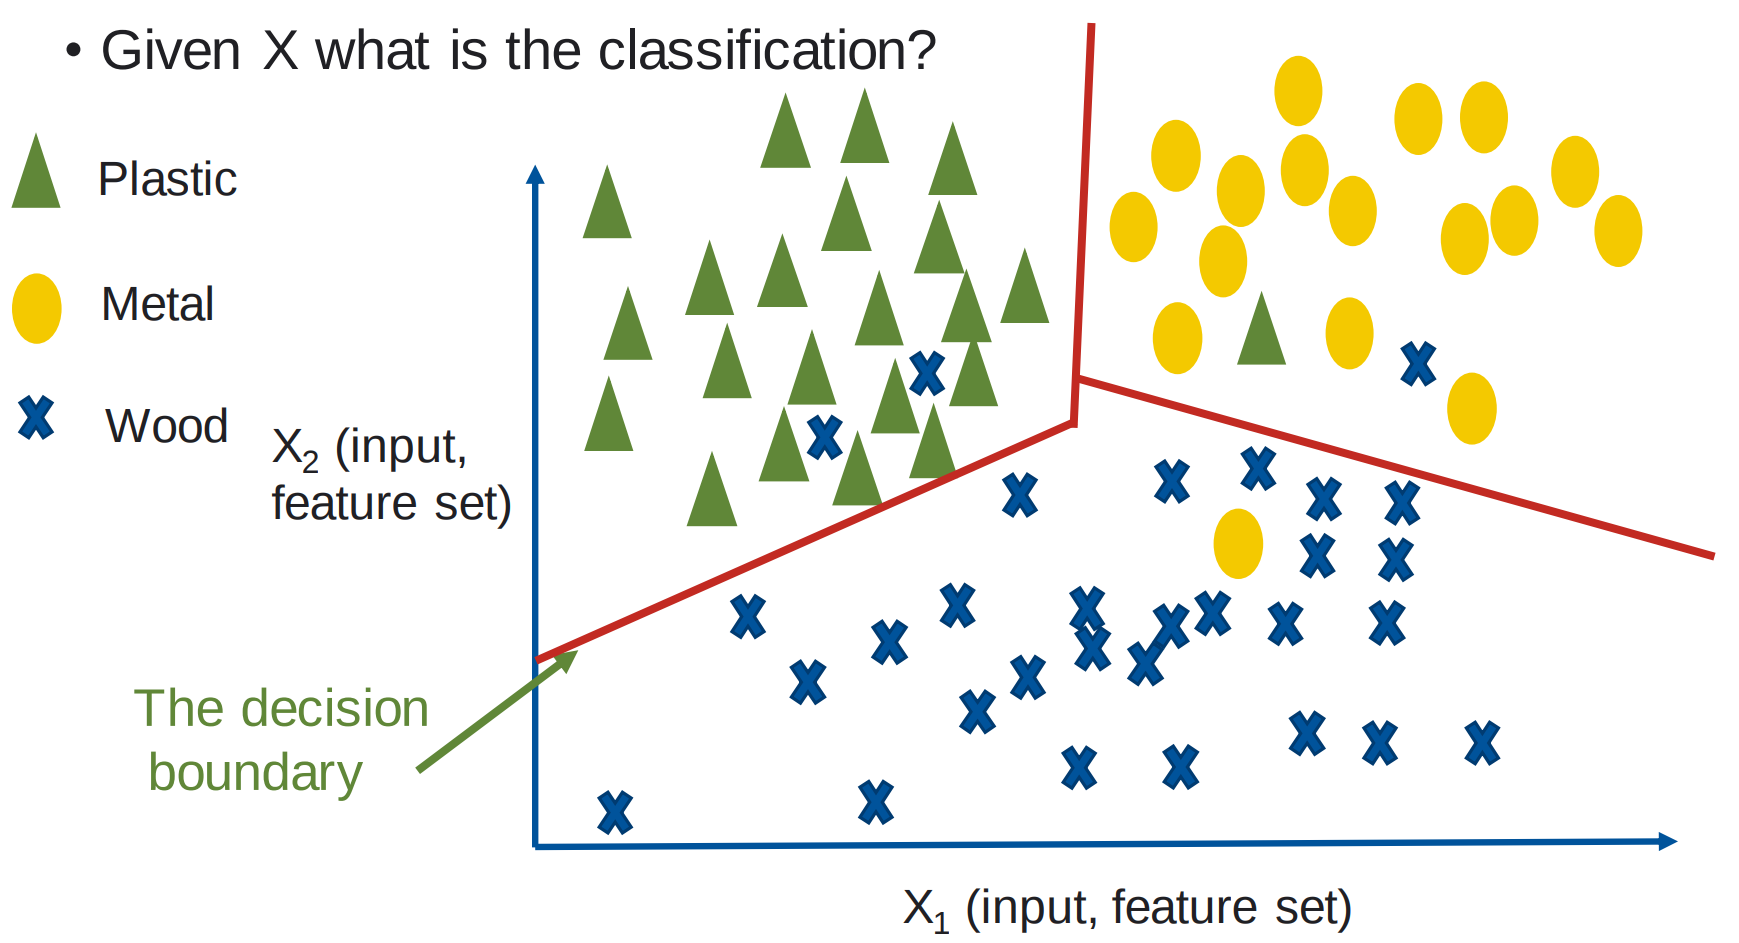
\includegraphics[width=0.9\textwidth, keepaspectratio]{imgs/classification-example.png}
\caption{Classification of 3 classes using 2 input features. Having more than 3 input features (3D plot) is difficult to visualise.}
\end{figure}
\noindent
One major issue with many machine learning algorithms: \textbf{overfitting}. Often the models trained become optimised too well towards the training data, leading to very low errors, but an inability to generalise to unseen data. 
\begin{figure}[H]
\centering
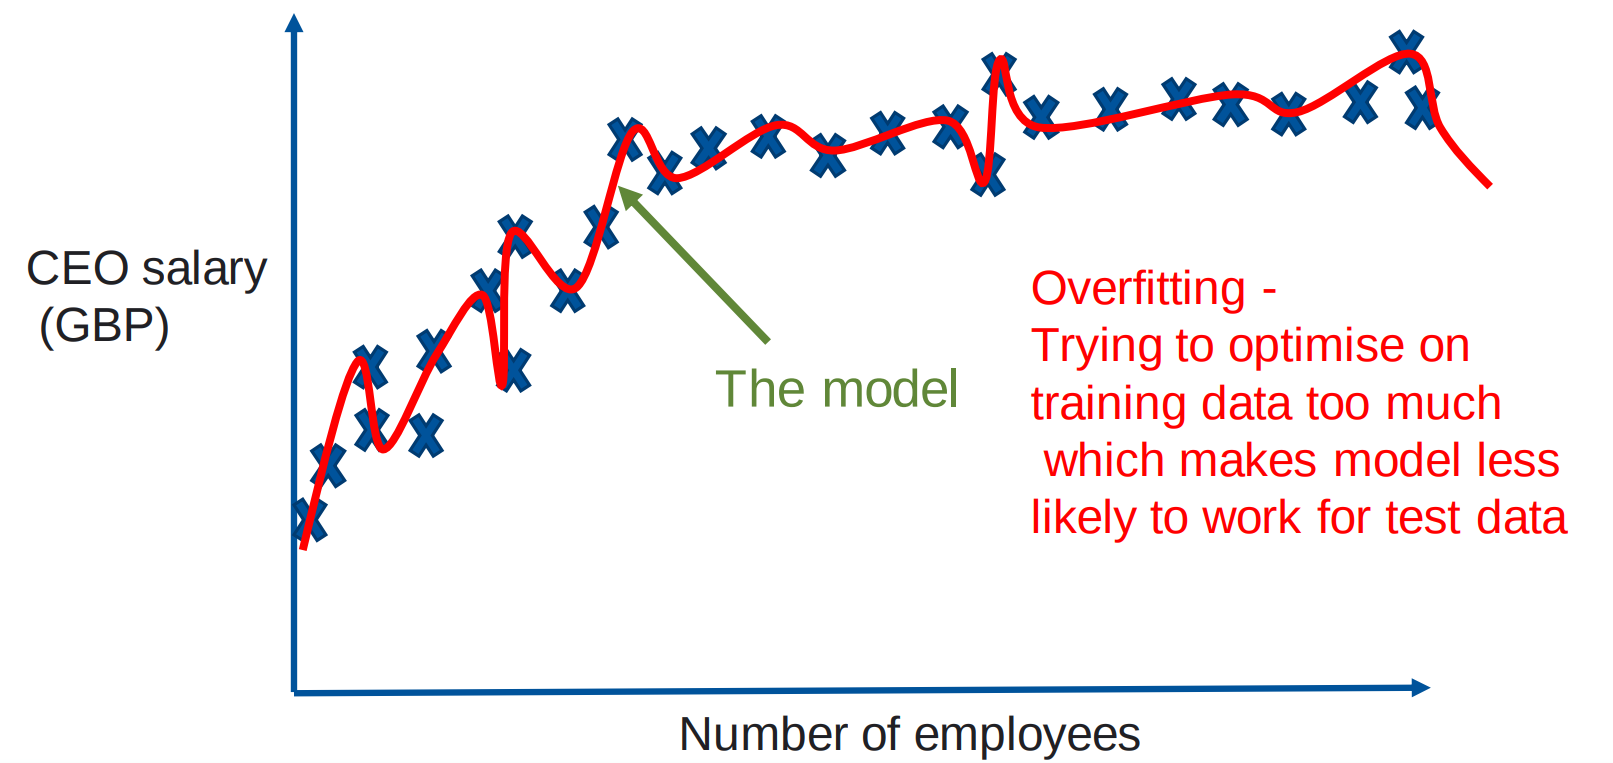
\includegraphics[width=1\textwidth, keepaspectratio]{imgs/overfitting-example.png}
\caption{Example of overfitting in linear regression.}
\end{figure}

\subsection{Unsupervised machine learning}
In unsupervised learning, the dataset is \textbf{unlabelled}, and the output for predicted values is unknown. To learn, clusters are automatically created to separate the data into distinct groups. This is useful for discovering information where we don't know what we are looking for or to discover things we don't know about.
\end{document}
